\chapter{Verifikácia predpovedných modelov počasia}

Verifikácia je proces, ktorý má overiť správnosť fungovania predpovedného modelu počasia. Z tohto dôvodu je nepostrádateľnou súčasťou meteorologického výskumu a taktiež celkového procesu predpovedania počasia \cite{MET:MET52}.
Ciele verifikácie môžeme rozdeliť do troch skupín: \textit{administratívne}, \textit{vedecké} a \textit{ekonomické}.
Medzi \textit{administratívne ciele} patrí monitorovanie úspešnosti predpovedania modelu a nasmerovanie užívateľov na jeho správnu konfiguráciu alebo voľbu iného modelu. \textit{Vedeckými cieľmi} sú identifikovanie a oprava slabín modelu a taktiež vylepšovanie predpovedí. \textit{Ekonomickými cieľmi} sú rozhodovanie, kam majú smerovať investície do výskumu a iné závažné ekonomické rozhodnutia \cite{IntroToVerif}. 

\section{Predpovedný model počasia}

Už v 19. storočí vývoj termodynamiky na základe Newtonovskej fyziky vyvrcholil v ucelení množiny fundamentálnych princípov, ktoré riadia prúdenie plynov v atmosfére. 
Začiatkom 20. storočia sa o matematický prístup k predpovedaniu počasia najviac zaslúžili osobnosti ako Vilhelm Bjerknes alebo Lewis F.Richardson. Avšak na ďalší úspech, v tejto oblasti, sa muselo čakať až na vynájdenie prvých počítačov počas 2. svetovej vojny ako bol IAS alebo ENIAC \cite{Origins}. Prvá úspešná predpoveď bola vykonaná v 50. rokoch minulého storočia a to hlavne vďaka práci Jula Charneyho.

Následný vývoj vo výpočtovej sile počítačov, používanie satelitných pozorovaní a vývoj samotnej meteorológie ako vedy zapríčinil, že je numerická predpoveď počasia (NWP) dnes najúspešnejším prístupom ako predpovedať počasie \cite{Golding}.  

Odvtedy vzniklo veľké množstvo modelov, ako sú napríklad GFS, NAM, RUC, WRF, SREF, GEFS, ECMWF, ALADIN a mnoho ďalších. Naša práca sa zameriava konkrétne na verifikáciu modelu \textit{WRF}. Taktiež pokračuje neustály vývoj aj vďaka novým modelovacím technikám, novým parametrizáciám, a zvyšovaniu výkonu výpočtových zdrojov.

\begin{figure}
	\centering
	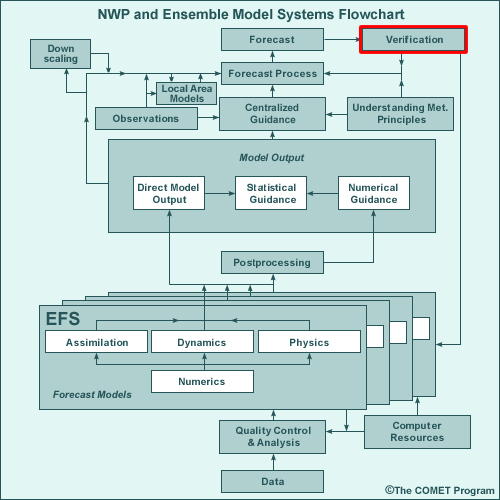
\includegraphics[width = 3.8in]{ForecastModelDiagramNew}
	\caption{Flowchart systému predpovedného model počasia od edukačného programu The COMET \cite{Comet}. Na obrázku je zvýraznená časť, ktorej sa venujeme v tejto práci.}
	\label{fig:fcstmodel}
\end{figure}

Ako môžeme vidieť na obrázku \ref{fig:fcstmodel} proces predpovedania počasia má okrem numerického modelu, ktorý je jej jadrom, aj iné časti. Ako príklad môžme spomenúť získavanie vstupných dát, ich predspracovanie, následné spracovanie, spracovanie výstupu a následne poskladanie samotnej predpovede. Cieľom nášho záujmu, celého procesu predpovedania, je \textit{verifikácia}. Ako môžme vidieť z obrázka, verifikácia vplýva na vyladenie parametrov modelu, avšak tento proces sa nedeje automaticky, ale vyžaduje prácu meteorológov a ich chápanie základných meteorologických princípov.

\subsection{WRF model}
\label{subsec:wrf}
Ako sme už spomenuli \textit{The Weather Research and Forecasting} (WRF) model je \textit{numerická predpoveď počasia} (NWP) a systém atmosferickej simulácie.

WRF je podporovaný, ako bežný nástroj pre univerzity, výskum a operačné komunity, pričom sa usiluje o splnenie všetkých ich požiadaviek súčasne.
Vývoj WRF modelu bol snahou mnohých spoločností ako napríklad \textit{The National Center for Atmospheric Research’s} (NCAR), \textit{Mesoscale and Microscale
Meteorology} (MMM), \textit{The National Oceanic and Atmospheric Administration’s} (NOAA) \textit{National Centers for Environmental Prediction} (NCEP) a \textit{Earth System Research Laboratory} (ESRL), oddelenie ministerstva obrany \textit{Air Force Weather Agency} (AFWA) a \textit{Naval
Research Laboratory} (NRL), \textit{The Center for Analysis and Prediction of Storms} (CAPS) \cite{WRF}. 

WRF model je vhodný pre širokú škálu aplikácií od \textit{metódy vzdušných vírov} (Large Eddy Simulation - LES) až po globálne simulácie počasia. Takéto aplikácie vyžadujú numerické predpovede v reálnom čase, vývoj a štúdium asimilácie dát, výskum parametrizovanej fyziky ,modelovanie kvality ovzdušia a idealizované simulácie, čo všetko WRF model spĺňa.

V roku 2008 evidovala WRF viac ako 6000 užívateľov, no dnes (2015) eviduje viac ako 25000 užívateľov vo viac ako 130 krajinách sveta. Tieto fakty poukazujú na to, že WRF model má nie len veľkú základňu užívateľov, ale aj vývojárov a má v budúcnosti istotne svoje miesto a preto si myslíme, že sa oplatí investovať čas a úsilie do verifikácie tohto modelu.

\section{Dáta}
\label{sec:data}
Na správne zhodnotenie úspešnosti modelu potrebujeme dva druhy dát. V prvom rade sa jedná o dáta, ktoré sú výstupom z daného predpovedného modelu počasia, teda \textbf{predpovedané dáta}. Tieto umelo získané dáta chceme konfrontovať s realitou, aby sme si mohli vytvoriť obraz o správnom fungovaní celého modelu. Realitu v našom prípade predstavujú dáta namerané špecializovanými meteorologickými senzormi, ktoré označujeme ako \textbf{pozorované dáta} alebo skrátene \textit{pozorovania}.  

\subsection{Predpovedané dáta}
Predpovedané dáta z modelu WRF sa ukladajú vo formáte \textbf{GRIB}, čo je skratka pre \textit{GRIdded Binary} \cite{GRIB} alebo na iných miestach uvádzané ako \textit{General Regularly-distributed Information in Binary form} \cite{GRIB12}. Tento formát je štandardom Svetovej meteorologickej organizácie teda \textit{World Meteorological Organization} (WMO). Jedná sa o pomerne rozšírený formát, používaný pri veľkom množstve meteorologických aplikácií a je taktiež používaný ako výstupný formát pre iné predpovedné modely ako WRF, či už ECMWF, GFS, NAM, SREF alebo mnohé ďalšie \cite{Products}.

Doteraz boli vyvinuté 3 verzie tohoto formátu od 0 po 2. Verzia 0 bola určená pre malé projekty typu TOGA a to iba s limitovaným použitím a dnes sa táto verzia už vôbec nepoužíva. Verzia grib 1 \cite{GRIB} a grib 2 \cite{GRIB12} sú dnes bežne používané väčšinou meteorologických centier.

Medzi verziami 1 a 2 nie sú žiadne rozdiely v obsahovej filozofii, preto popis obsahu gribovského formátu, ktorý tu uvádzame je spoločný pre obe tieto verzie. 
\textit{Gribovský súbor} (ďalej iba \textit{Grib}) pozostáva z viacerých \textit{Gribovských záznamov}, pričom jeden záznam môže existovať ako samostatný Grib. Vďaka tomu je možné ľahko spájať Griby, a to tiež v ľubovoľnom poradí, bez toho, aby sme ich nejako poškodili. Samozrejme musí byť zachovaná homogenita, čo sa týka verzií Gribov, teda verziu 1 nemožno miešať s verziou 2 a naopak.
Už samotný názov \textit{Gridded Binary} nám napovedá, že dáta sú usporiadané v pravidelnej mriežke. Každý Gribovský záznam obsahuje dvojrozmernú mriežku (zemepisná šírka x zemepisná dĺžka) hodnôt v určitom čase a vertikálnej hladine. Taktiež v hlavičke záznamu sa nachádzajú \textit{meta-informácie}, ktoré nám hovoria o aké dáta ide, teda o akú premennú sa jedná, čas predpovede, výškovú hladinu a podobne. Grib je zvyčajne z tohto dôvodu 2 až 5 rozmerná dátová štruktúra s veľkým množstvom veličín ako je napríklad teplota, tlak, relatívna vlhkosť, rosný bod, \textit{u} a \textit{v} súradnice vetra a ďalšie, ktoré sú definované v rôznych hladinách. Taktiež je dôležité povedať, že Grib zriedkakedy zachytáva povrch celej planéty, ale iba vymedzenú skúmanú oblasť - \textit{doménu}.

\subsection{Pozorované dáta}
Pozorovania sa získavajú meraním priamo v teréne pomocou špecializovaných meracích zariadení, ktoré sú súčasťou meteo staníc. Každá stanica môže obsahovať iné vybavenie, ku príkladu teplomer, zrážkomer, barometer, vetromer a im podobné \cite{WeatherStation}, ktorými môžme zachytávať informácie o rôznych skúmaných veličinách. 
%http://www.weathergraphics.com/dl/obsman.pdf
% http://en.wikipedia.org/wiki/Weather_station

Majoritná časť meraní sa deje pri povrchu zeme priamo na meteo staniciach a nazývajú sa \textit{surface} merania. Tieto merania najlepšie popisujú dianie v oblasti najväčšieho záujmu (biosfére), avšak neobsahujú informáciu o dianí v iných výškových hladinách. Pozorovania týchto hladín sa dejú pomocou \textit{radiosondy}, ktorá je pripojená k meteo balónu alebo vypustená z lietadla smerom k zemi. Takéto pozorovania sa nazývajú \textit{upper air} merania.

Narozdiel od predpovedaných dát, pozorované dáta nemajú štandardizovaný formát a zvyčajne sa ukladajú do databázy.
Aby sme zhrnuli charakteristiku týchto dát, jedná sa o niekoľko meraných veličín, nameraných v konštantných časových krokoch - napríklad každú minútu alebo každú hodinu - v jednom konkrétnom geografickom bode a zvyčajne pri povrchu zeme, teda ak sa nejedná o upper air merania, ktoré sa uskutočňujú v štandardných výškových hladinách, ktoré sa merajú v hPa.

\subsection{Párovanie dát}
\label{subsec:pairing}
%TODO novy pristup
Z predpovedného modelu a rovnako aj z merania získame veľké množstvo hodnôt. Aby sme mohli korektne porovnať predpovede s pozorovaniami, je nevyhnutné nájsť správne párovanie týchto hodnôt, teda zistiť, ktorú hodnotu porovnať s ktorou, aby sme získali zmysluplný výsledok.

Vždy sa snažíme nájsť správnu predpoveď pre pozrovanie a nie naopak.
% Vzhľadom na charakter dát sa 
Dôvodom je, že chceme skúmať vzťah predpovede s realitou a preto v párovaní musí byť zahrnutých čo najviac \textbf{meraných} hodnôt, ak nie všetky.

Každá pozorovaná hodnota, ktorú chceme spárovať má štyri kľúče podľa ktorých hľadáme pár: \textit{meraná veličina} (napríklad teplota), \textit{čas merania}, \textit{výšková hladina} a \textit{geografická poloha}.
Nájsť všetky hodnoty podľa kľúča meranej veličiny v Gribe je ľahké, keďže sa jedná o kategorickú premennú, teda môže nadobúdať iba určitý konečný počet hodnôt. Toto sa však nedá povedať o čase, hladine a polohe, ktoré sú spojitými premennými.
 
Pre čas pozorovania, čas predpovede a výškovú hladinu existujú štandardy, ktoré určujú v akých časoch resp hladinách sa robia merania a predpovede, čo nám uľahčuje prácu. Ak sa napriek tomu čas alebo hladina v Gribe nevyskytuje, tak pár vyhadzujeme z párovania. 

V prípade polohy zo samozrejmých dôvodov neexistuje žiaden štandard a hustota mriežky v Gribe nemôže byť nikdy tak veľká, aby poloha našej stanice vždy dopadla na presný bod mriežky. Z tohoto dôvodu získavame hodnoty z mriežky z okolitých bodov a to dvoma metódami \textit{Point-to-Grid} a \textit{Grid-to-Point} \cite{IntroToVerif}, ktoré sú znázornené na obrázku \ref{fig:pointmethods}. Jedná sa vlastne o dve interpolačné metódy. Point-to-Grid predstavuje metódu \textit{najbližší sused} (\textit{Nearest Neighbour}) a Grid-to-Point \textit{bilineárnu interpolačnú metódu}. 

Výber správnej metódy môže značne ovplyvniť výsledok. Dôvodom je, že môžu byť veľké rozdiely hodnôt v okolitých mrežových bodoch a tak, ak pomocou Point-To-Grid metódy získame nízku hodnotu, tak pomocou Grid-To-Point môžeme získať hodnotu omnoho väčšiu, vplyvom zvyšných troch bodov, ktoré vstúpili do interpolácie. Nemožno však jednoznačne povedať, ktorá z metód je lepšia, keďže obe môžu v istých prípadoch dávať lepšie výsledky. 

\begin{figure}
	\centering
	\begin{tabular}{ c c }
	\subfloat[Point-to-Grid]{\includegraphics[width = 2.5in]{PointtoGrid}} &
	\subfloat[Grid-to-Point]{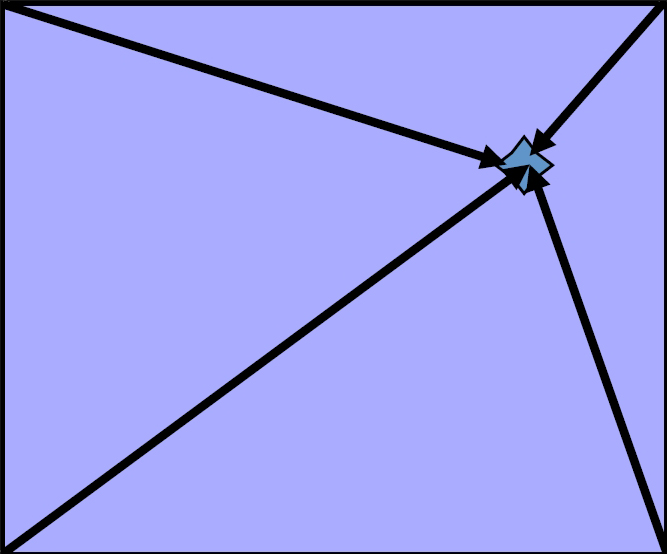
\includegraphics[width = 2.5in]{GridToPoint}} 
	\end{tabular}

	\caption{Vizuálne znázornenie dvoch bežne používaných metód na získavanie hodnôt z mriežky}
	\label{fig:pointmethods}
\end{figure}


\section{Metódy verifikácie}
Metódy verifikácie sa delia podľa typu predpovede na 3 druhy \cite{RecommendOnVerif}: 
\begin{easylist}[itemize]
	# Verifikácia predpovede spojitých premenných
	# Verifikácia kategorickej predpovede
	## Dichotomické (áno/nie) predpovede
	## Mnoho-kategorické predpovede
	# Verifikácia pravdepodobnostných predpovedí
\end{easylist}

\section{Meranie chyby predpovede}
\label{sec:errormeasurement}
Výsledkom procesu párovania je $n$ párov (predpoveď, pozorovanie), ktoré je možné porovnať. Z porovnania týchto dvojíc získame numerickú hodnotu, ktorá nám hovorí o veľkosti chyby predpovede daného modelu pre vybrané predpovedané časy.
\\
Chybu predpovede $e_i$ pre $i$-tu dvojicu $(y_i, \hat{y}_i)$ definujeme takto: 
\[  
	e_i = (y_i - \hat{y}_i)
\]
Kde $ y_i $ je predpoveď a $ \hat{y}_i $ je pozorovanie.
Takýmto spôsobom z $ n $ párov získame $ n $ chýb, ktoré agregujeme pomocou rôznych štatistických metód, ktoré sú bežne používané pri verifikácií predpovedí, ako sa spomína v \cite{RecommendOnVerif}, \cite{IntroToVerif} a \cite{ContinuousVerif}. Výsledkom agregácie je numerická hodnota, ktorá sa nazýva \textit{skóre} predpovede. 

\subsection{Stredná chyba predpovede}
Budeme ju označovať ako \textit{MFE} z anglického \textit{Mean Forecast Error}, ale v literatúre je možné ju nájsť ako \textit{ME} \cite{RecommendOnVerif}, teda \textit{stredná chyba} alebo ako \textit{Linear Bias} \cite{ContinuousVerif}, \cite{IntroToVerif}. Vzorec pre výpočet MFE vyzerá nasledovne:
\[
	MFE = \frac{1}{n}\sum\limits_{i=0}^{n}  e_i  
\]
MFE je možné vypočítať aj ako rozdiel priemerov predpovedí a pozorovaní.
\[
	MFE = \bar{y} - \bar{\hat{y}}  
\]
MFE vyjadruje priemerný smer chyby. To znamená, že pozitívny výsledok indikuje \textit{over-forecast}, teda nadhodnotenú predpoveď a negatívny výsledok \textit{under-forecast}, teda podhodnotenú predpoveď. Avšak MFE \textbf{nevyjadruje veľkosť} chyby v tomto smere, keďže kladné a záporné chyby sa navzájom môžu zrušiť. 
Napríklad máme množinu chýb $ E = \{2, -5\} $, tak MFE pre $ E $ je -1.5, ale priemerná veľkosť chyby je 3.5.  

\subsection{Stredná absolútna chyba}
Budeme ju označovať ako \textit{MAE} z anglického \textit{Mean Absolute Error}. Vzorec pre výpočet MAE vyzerá nasledovne:
\[
	MAE = \frac{1}{n}\sum\limits_{i=0}^{n} \lvert e_i \rvert 
\]
Narozdiel od MFE \textbf{neurčuje smer chyby}, ale vyjadruje veľkosť chyby. Z týchto dôvodov je v praxi odporúčané zobrazovať MFE a MAE súčasne \cite{RecommendOnVerif}. 

\subsection{Stredná kvadratická chyba}
Budeme ju označovať ako \textit{RMSE} z anglického \textit{Root Mean Square Error}. Vzorec pre výpočet RMSE vyzerá nasledovne:
\[
	RMSE = \sqrt{ \frac{1}{n}\sum\limits_{i=0}^{n} e_i^{2}  }
\]
Z povahy vzorca pre RMSE je jasné, že rovnako ako MAE, ani RMSE neurčuje smer chyby, pretože nadobúda vždy iba kladné hodnoty. 
Ďalšou vlastnosťou RMSE je, že nadobúda hodnoty vždy väčšie alebo rovné ako MAE, pričom výsledok RMSE je citlivý na veľké hodnoty chýb. \\
\label{subsec:mse}
V praxy sa zvykne používať aj \textit{MSE} (\textit{Mean Square Error}):
\[
	MSE = \frac{1}{n}\sum\limits_{i=0}^{n} e_i^{2} 
\]
Má podobné vlastnosti ako RMSE s jediným rozdielom, že RMSE meria veľkosť chyby zachovávajúc jednotky danej veličiny (napr. \textcelsius), zatiaľ čo MSE jednotky nezachováva \cite{RecommendOnVerif}. Preto sme si pre náš účel zvolili RMSE, ktoré je jednoduchšie zobraziť spolu s MFE a MAE v jednom grafe, keďže sa zachováva konzistentnosť jednotiek veličín.



%\subsection{Signál chybných predikcií}
%\[ 
%	TS = \frac{\sum\limits_{i=0}^{n} e_i}{MAE}
%\]

\subsection{Všeobecná kumulovaná chyba}
\label{subsec:cumulativeerror}
V našom systéme sme navrhli všeobecný vzorec na výpočet kumulovaného skóre, ktorým možno vyjadriť ľubovoľnú zo spomenutých štatistických metód. Takéto vyjadrenie umožňuje nie len všeobecnosť, ale aj jednoduché rozšírenie systému o ďalšie metódy a to nie len programátorom, ale aj samotným užívateľom systému.
\\
Všeobecný vzorec na výpočet \textit{skóre} pre danú predpoveď vyzerá takto:
\[
	Score = \Phi(\sum\limits_{i=0}^{n} \varepsilon(e_i))  
\]
Kde $ \Phi $ je ľubovoľná funkcia z $\mathbb{R}$ do $\mathbb{R}$, teda $ \Phi : \mathbb{R} \rightarrow \mathbb{R} $ a podobne funkcia $ \varepsilon : \mathbb{R} \rightarrow \mathbb{R} $.
Spomenuté metódy môžme teda skonštruovať zadefinovaním správneho $ \Phi $ a $ \varepsilon $. \\
Napríklad pre \textit{MFE}:
\[ \Phi(x) = \frac{x}{n} \]
\[ \varepsilon(e) = e \] 
Pre \textit{MAE}:
\[ \Phi(x) = \frac{x}{n} \]
\[ \varepsilon(e) = \lvert e \rvert \]
Pre \textit{RMSE}:
\[ \Phi(x) = \sqrt{\frac{x}{n}} \]
\[\varepsilon(e) = e^2 \]
Pre \textit{MSE}:
\[ \Phi(x) = \frac{x}{n} \]
\[ \varepsilon(e) = e^2 \] 

Ako sme spomenuli, je možné rozšírenie o ďalšie metódy a to napríklad o Brownov a Triggov \textit{signál chybných predikcií}, ktorý budeme označovať ako \textit{TS} z anglického \textit{Tracking Signal}. Tieto metódy sme vyššie nespomenuli, keďže sa v meteorologickej praxi nepoužívajú. Uvádzame ich však ako možné rozšírenie, keďže sú tieto metódy bežne používané pri verifikácii iných predpovedných modeloch, ako sú tie meteorologické.

\subsection{Medián absolútnych chýb}
\label{subsec:mad}
Budeme ju označovať ako \textit{MAD} z anglického \textit{Median Absolute Deviation}. Vzorec pre výpočet MAD vyzerá nasledovne:
\[
	MAD = median( \lvert e  \rvert) = \tilde{ \lvert e  \rvert}
\]
Nech je daná usporiadaná postupnosť $ Y_1, \ldots , Y_N $, tak potom $ median $ náhodnej premennej $ x $ je definovaný rovnako ako v \cite{StatMedian}:
\[
	median(x) = \tilde{x} \equiv \left\{
		\begin{array}{ll}
			Y_{(N+1)/2}  & \mbox{ak } N\mod{2} = 0 \\
			\frac{1}{2}(Y_{(N+1)/2} + Y_{(N+1)/2 + 1}) & \mbox{ak } N\mod{2} = 1
		\end{array}
	\right.
\]
Z daného vzorca môžeme vidieť podobné vlastnosti ako má MAE, avšak MAD je robustnejší a extrémne chyby nemajú na skóre žiaden efekt.

%TODO pridat LEPS - http://www.cawcr.gov.au/projects/verification/LEPS.php
% preto treba aj zmenit nejake veci 